% !TEX root = handbook-physics.tex
%!TEX TS-program = pdflatex
%!TEX encoding = UTF-8 Unicode

\chapter{First law of Thermodynamics}
\label{ch-09}
\zhtitle{热力学第一定律}


\section[Total and Internal Energy]{Total and Internal Energy of a System}
\label{sec-9.1}
\zhtitle{系统的总能量与内能}

\subsection{}\label{9.1.1} An arbitrary thermodynamic system \ssect{8.3.1}, in any thermodynamic state \ssect{8.3.3}, has a \redem{total energy} $E$ , which is the sum of:
\zhpar{任一热力学系统 \ssect{8.3.1}，处于任意热力学状态 \ssect{8.3.3} 时，都具有\redem{总能量} $E$，它是以下各项之和：}
\begin{enumerate}[label=(\alph*)]
\item the kinetic energy $E_{k}^{\textrm{Mech}}$ of mechanical motion of the system
as a whole (or of its macroscopic parts);
\zhpar{系统作为一个整体（或其宏观部分）的机械运动动能 $E_{k}^{\textrm{Mech}}$；}
\item the potential energy $E_{p}^{\textrm{Ext}}$ \ssect{3.3.1} of the system in all external force fields (for instance, electromagnetic or gravitational fields); and
\zhpar{系统在各外力场（例如电磁场或引力场）中的势能 $E_{p}^{\textrm{Ext}}$ \ssect{3.3.1}；以及}
\item the internal energy U:
\zhpar{系统的内能 U：}
\begin{equation*}%
E = E_{k}^{\textrm{Mech}} + E_{p}^{\textrm{Ext}} + U.
\end{equation*}
\end{enumerate}

\subsection{}\label{9.1.2} The \redem{internal energy} of a body or of a thermodynamic system \ssect{8.3.1} is the energy depending only upon the thermodynamic state of the body (or system). For a fixed (stationary) system, not located in any external force fields, the internal energy coincides with the total energy. The internal energy also coincides with the rest energy of a body (or system) \ssect{5.7.3} and includes the energy of all the types of internal motion of a body (or system) and the energy of interaction of all the particles (atoms, molecules, ions, etc.) making up the body (or system).
\zhpar{物体或热力学系统的\redem{内能}是仅取决于该物体（或系统）热力学状态的能量。对于静止的固定系统（不处于任何外力场中），内能与总能量相等。内能也等于物体（或系统）的静止能量 \ssect{5.7.3}，并包括物体（或系统）内部各种运动形式的能量，以及构成物体（或系统）的所有粒子（原子、分子、离子等）之间相互作用的能量。}

For example, the internal energy of a gas consisting of poly­ atomic molecules (ammonia, carbon dioxide, etc.) consists of: 
\zhpar{例如，由多原子分子（氨、二氧化碳等）组成的气体，其内能包括：}
\begin{enumerate}[label=(\alph*)]
\item kinetic energy of thermal translational and rotary motion of the molecules;
\zhpar{气体分子热运动中平动和转动的动能；}
\item kinetic and potential energy of vibration of the atoms and molecules;
\zhpar{原子和分子振动的动能与势能；}
\item potential energy due to intermolecular interactions;
\zhpar{分子间相互作用的势能；}
\item energy of the electron shells of the atoms and ions;
\zhpar{原子和离子的电子壳层的能量；}
\item kinetic energy and potential energy of interaction of the nucleons \ssect{42.1.1} in the nuclei of the atoms.
\zhpar{原子核中核子 \ssect{42.1.1} 之间相互作用的动能与势能。}
\end{enumerate}
Terms (d) and (e) do not ordinarily change in processes that proceed at not very high temperatures so that ionization and excitation play no essential role. Under these conditions, terms (d) and (e) are not taken into account in the internal energy balance. Term (c) is also neglected for an ideal gas \ssect{8.4.1}.
\zhpar{在温度不太高、电离和激发不起实质性作用的过程中，第 (d) 项和第 (e) 项通常不发生变化。在这种条件下，第 (d) 项和第 (e) 项不计入内能的平衡。对于理想气体 \ssect{8.4.1}，第 (c) 项也可忽略。}

\subsection{}\label{9.1.3} The internal energy is a single-valued function of the thermodynamic state of a system. The value of the internal energy in any state is independent of the process by means of which the system reached this state. The change in internal energy in the transition of a system from state \hlblue{1} to state \hlblue{2} equals $\Delta U = U_{2} - U_{1}$ and is independent of the kind of transition $\hlblue{1} \to \hlblue{2}$ that occurs. If the system accomplishes a cycle \ssect{11.1.1} the total change in its internal energy is equal to zero: 
\zhpar{内能是热力学系统状态的单值函数。系统在任一状态下的内能值，与系统达到该状态所经历的过程无关。系统从状态\hlblue{1}过渡到状态\hlblue{2}时，内能的变化为 $\Delta U = U_{2} - U_{1}$，它与过渡 $\hlblue{1} \to \hlblue{2}$ 的具体方式无关。若系统完成一个循环 \ssect{11.1.1}，则其内能的总变化等于零：}
\begin{equation*}%
\oint \dd U = 0.
\end{equation*}
As is well known, such a relation mathematically signifies that an element of change in the internal energy $\dd U$ is a com­plete (exact) differential. This property is also possessed by the entropy \ssect{11.4.2} and other state functions \ssect{8.3.8} (cf. \ssect{9.2.5}). 
\zhpar{众所周知，从数学上看，这一关系表明内能的变化元 $\dd U$ 是一个全（恰当）微分。熵 \ssect{11.4.2} 以及其他状态函数 \ssect{8.3.8} 也具有这一性质（参见 \ssect{9.2.5}）。}

\subsection{}\label{9.1.4} In a system that is in a state of thermodynamic equilibrium the internal energy depends only upon the temperature and the external variables \ssect{8.3.5}. In particular, for a simple system \ssect{8.3.6} of constant mass $M$, the internal energy is a func­tion of the temperature $T$ and volume $V$ of the system (\redem{calorific equation of state} of a simple system):
\zhpar{在处于热力学平衡态的系统中，内能仅取决于温度和外部参量 \ssect{8.3.5}。特别地，对于质量 $M$ 保持不变的简单系统 \ssect{8.3.6}，其内能是系统温度 $T$ 和体积 $V$ 的函数（简单系统的\redem{量热物态方程}）：}
\begin{equation*}%
U= \varphi (V, \,T).
\end{equation*}

\noindent\hlblue{Example 1.} The internal energy of an ideal gas \ssect{8.4.1} depends only on its absolute temperature and is proportional to the mass $M$ of the gas:
\zhpar{\hlblue{例 1.} 理想气体 \ssect{8.4.1} 的内能仅取决于其绝对温度，并与气体的质量 $M$ 成正比：}
\begin{equation*}%
U = \oint_{0}^{T} C_{V} \dd T + U_{0}= M \left(\oint_{0}^{T} c_{V} \dd T + u_{0}\right).
\end{equation*}
where $C_{V}$ and $c_{V} = C_{V}/M$ are the heat capacity \ssect{9.5.1} and specific heat \ssect{9.5.2} of the gas at constant volume (in an isochoric process) \ssect{8.3.7}, $u_{0} = U_{0}/M$ is the internal energy of unit mass of the gas at $T = \SI{0}{\kelvin}$. For monatomic gases at ordinary temperatures $C_{V}$ is independent of $T$, and $U = C_{V}T + U_{0}$. 
\zhpar{式中 $C_{V}$ 和 $c_{V} = C_{V}/M$ 分别为气体在定容（等体过程）条件下的热容 \ssect{9.5.1} 和比热容 \ssect{9.5.2}，$u_{0} = U_{0}/M$ 为 $T = \SI{0}{\kelvin}$ 时单位质量气体的内能。对于常温下的单原子气体，$C_{V}$ 与温度无关，此时 $U = C_{V}T + U_{0}$。}

\noindent\hlblue{Example 2.} The internal energy of a van der Waals gas \ssect{12.2.1} is:
\zhpar{\hlblue{例 2.} 范德瓦耳斯气体 \ssect{12.2.1} 的内能为：}
\begin{equation*}%
U = \oint_{0}^{T} C_{V} \dd T - \frac{M^{2}}{\mu^{2}} \frac{a}{V} + U_{0},
\end{equation*}
where $M$ is the mass of the gas, $\mu$ is its molar mass \ssect{8.4.3}, and $a$ is the van der Waals' coefficient \ssect{12.2.3}.
\zhpar{式中 $M$ 为气体的质量，$\mu$ 为其摩尔质量 \ssect{8.4.3}，$a$ 为范德瓦耳斯常量 \ssect{12.2.3}。}

\subsection{}\label{9.1.5} In thermodynamics, the internal energy is determined to an accuracy of the constant term $U_{0}$, whose value depends upon the choice of the reference point for the quantity $U$, i.e. from a state with zero internal energy. The quantity $U_{0}$ plays practically no role in thermodynamical calculations in which the changes $\Delta U$ of internal energy, independent of $U_{0}$, are determined (see also \ssect{8.1.2}).
\zhpar{在热力学中，内能只能确定到常数项 $U_{0}$ 的精度，该常数的值取决于 $U$ 的参考点的选取（即从内能为零的状态算起）。在热力学计算中，$U_{0}$ 实际上不起作用，因为只需确定与 $U_{0}$ 无关的内能变化 $\Delta U$（另见 \ssect{8.1.2}）。}

\section{Heat and Work}
\label{sec-9.2}
\zhtitle{热量与功}

\subsection{}\label{9.2.1} An energy exchange between a thermodynamic system and external bodies takes place in two ways: either by doing work or by means of heat exchange.\sidenote{A discussion of the third way of energy exchange -- mass trans­fer -- is beyond the scope of the present handbook.} The amount of energy transferred to the system by external bodies in force inter­ action between the system and the bodies is called \redem{work} done on the system. The amount of energy transferred to the system by external bodies by heat transfer is called the \redem{quantity of heat} imparted to the system.\sidenote{Sometimes the term ``heat'' is employed in place of the term ``quantity of heat'' if this leads to no confusion. It should be indicated, however, that heat, generally speaking, is to be under­ stood as a form of energy transfer \ssect{9.2.4}).}
\zhpar{热力学系统与外界物体之间的能量交换通过两种方式实现：做功或热交换。外界物体通过与系统之间的力的相互作用传递给系统的能量，称为外界对系统所做的\redem{功}；外界物体以热传递的方式传递给系统的能量，称为传递给系统的\redem{热量}。}
\zhpar{注：能量交换的第三种方式——质量传递——不在本手册的讨论范围之内。}
\zhpar{注：在不致引起混淆的情况下，有时用“热”代替“热量”一词。但应当指出，一般而言，“热”应理解为能量传递的一种形式（参见 \ssect{9.2.4}）。}

\subsection{}\label{9.2.2} If the thermodynamic system is fixed (stationary), a neces­ sary condition to do work is displacement of the external bodies interacting with it, i.e. it is necessary to change the external state variables of the system \ssect{8.3.5}. In the absence of external force fields, energy exchange between the lixed system and the external medium may take place by doing work when the volume and shape of the system are changed. According to the law of conservation of energy, the work $W'$ done on the system by external forces is numerically equal and opposite in sign to the work $W$ that the system does on the external medium, i.e. against the external forces:
\zhpar{若热力学系统是固定的（静止的），则要使其做功，必要条件是与其相互作用的外界物体发生位移，即必须改变系统的外部状态参量 \ssect{8.3.5}。在没有外力场的情况下，系统与固定系统外部介质之间的能量交换可以通过系统体积和形状的改变做功来实现。根据能量守恒定律，外力对系统所做的功 $W'$，在数值上等于系统对外部介质（即克服外力）所做的功 $W$，但符号相反：}
\begin{equation*}%
W' = -W.
\end{equation*}
\subsection{}\label{9.2.3} \redem{Expansion work} is the work done by the system in over­ coming the external pressure. An element of expansion work $\delta W = p_{\textrm{ext}} \dd V$, where $p_{\textrm{ext}}$ is the uniformly distributed external pressure, and dV is an element of change of the system's volume. If the expansion process is an equilibrium (quasistatic) one \ssect{8.3.7}, $p_{\textrm{ext}} = p$, where $p$ is the pressure in the system. Then $\delta W = p \dd V$.
\zhpar{\redem{膨胀功}是系统为克服外部压强所做的功。膨胀功元为 $\delta W = p_{\textrm{ext}} \dd V$，其中 $p_{\textrm{ext}}$ 为均匀分布的外部压强，$\dd V$ 为系统体积的变化元。若膨胀过程是平衡（准静态）过程 \ssect{8.3.7}，则 $p_{\textrm{ext}} = p$，其中 $p$ 为系统内的压强，于是 $\delta W = p \dd V$。}

The significance of the different ways used in denoting the elements of change $\delta W$ and $\dd U$ is explained in \ssect{9.4.3} and \ssect{9.1.3}. The work done in equilibrium expansion of system from volume $V_{1}$ to volume $V_{2}$ is
\zhpar{关于变化元 $\delta W$ 与 $\dd U$ 的不同记号的含义，参见 \ssect{9.4.3} 和 \ssect{9.1.3}。系统在平衡膨胀过程中由体积 $V_{1}$ 变化到体积 $V_{2}$ 时所做的功为：}
\begin{equation*}%
W = \int_{V_{1}}^{V_{2}} p \dd V.
\end{equation*}
\begin{marginfigure}%[!ht]
%\begin{wrapfigure}{r}{0.5\linewidth}
\centering
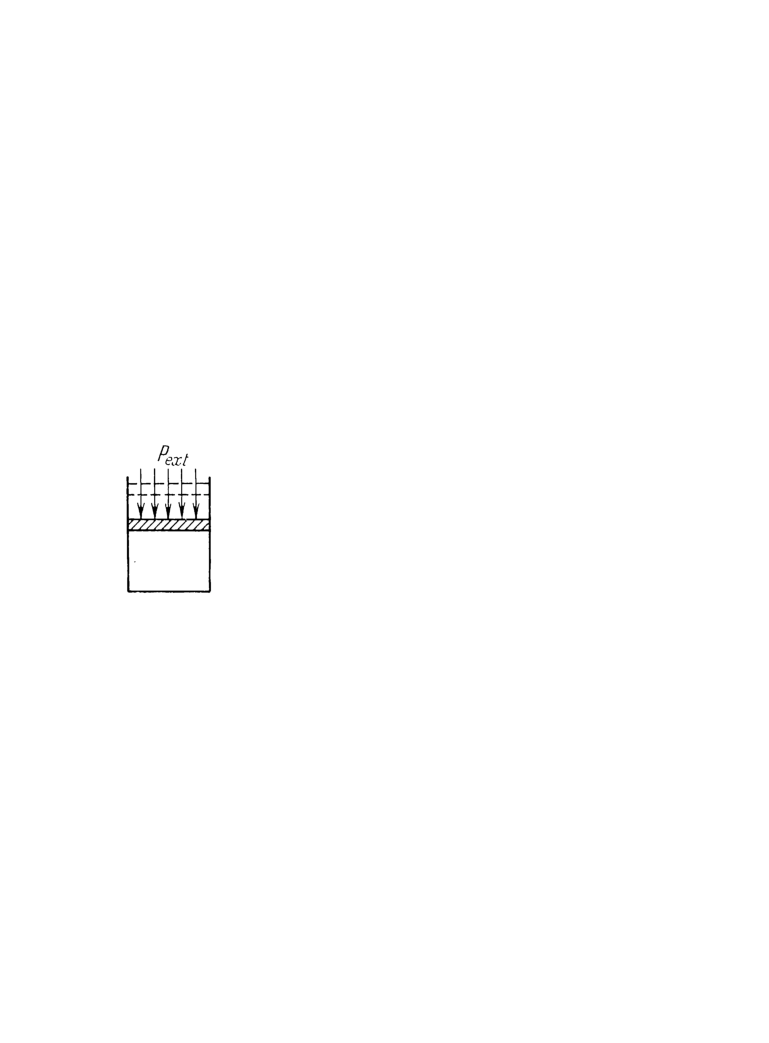
\includegraphics[width=0.5\textwidth]{figs/ch-09/fig-09-01.pdf}
%\input{figs/ch-03/fig-03-01}
%  \vspace{-13pt}
\sidecaption{The work done by a gas in a vessel with a weightless movable piston.\zhcap{气体在带有无重可动活塞的容器中所做的功。}\label{fig-09-01}}
\end{marginfigure}

\hlblue{Example.} The work done by a gas in a vessel with a weightless movable piston (\figr{fig-09-01}). The pressure of the gas $p > 0$ and, therefore, in its expansion $(\dd V > 0)$ the gas performs positive work $(\delta W > 0)$. In compressing the gas ($\dd V< 0$ and $\delta W < 0$) the positive work is done on the $p_{\textrm{ext}}$ gas by the forces of external pressure. Here the gas does negative work. The graphical representation of work is dis­cussed in \ssect{9.4.2}.
\zhpar{\hlblue{例.} 气体在带有无重可动活塞的容器中所做的功（见 \figr{fig-09-01}）。气体的压强 $p > 0$，因此在气体膨胀（$\dd V > 0$）时，气体做正功（$\delta W > 0$）。压缩气体（$\dd V < 0$，$\delta W < 0$）时，外部压力对气体做正功，此时气体做负功。功的图示表示方法参见 \ssect{9.4.2}。}



\subsection{}\label{9.2.4} Heat exchange takes place between bodies (or parts of bodies) heated to different temperatures. There are three types of heat exchange: convection, conduction and radiation (radiative heat exchange).
\zhpar{热交换发生在温度不同的物体（或物体的各部分）之间。热交换有三种类型：对流、热传导和辐射（辐射热交换）。}

\redem{Convective heat exchange} is the transfer of energy in the form of heat between the unequally heated parts of gases or liquids
or between gases, liquids and solids. Convective heat exchange in liquids takes place by motion of parts of the liquid with respect to one another or with respect to solids. For instance, in a radiator of a hot-water heating system, energy of the hot water flowing through the radiator is transferred by convection to the less heated walls of the radiator.
\zhpar{\redem{对流热交换}是指气体或液体中受热不均匀的各部分之间，或气体、液体与固体之间，以热的形式进行的能量传递。液体中的对流热交换是通过液体各部分相对于彼此或相对于固体的运动来实现的。例如，在热水采暖系统的散热器中，流经散热器的热水的能量通过对流传递给温度较低的散热器壁。}

The phenomenon of \redem{heat conduction} consists in the transfer of energy in the form of heat from one part of a non-uniformly heated body to another part. Thus, for example, energy is transferred through the walls of a heating radiator from the more heated inner surfaces to the less heated outer sur­faces.
\zhpar{\redem{热传导}现象是指能量以热的形式从非均匀受热物体的一部分传递到另一部分。例如，能量通过散热器的壁面，从温度较高的内表面传递到温度较低的外表面。}

\redem{Radiative heat exchange} takes place without direct contact of the bodies exchanging energy and consists in the emission and absorption of the energy of an electromagnetic field by the bodies. An immense amount of energy is delivered from the sun to the earth's surface by radiative heat exchange.
\zhpar{\redem{辐射热交换}不需要进行能量交换的物体直接接触，它通过物体对电磁场能量的发射和吸收来实现。通过辐射热交换，太阳向地球表面输送了巨大的能量。}

\subsection{}\label{9.2.5} Work and heat are the energy characteristics of processes for changing the state of thermodynamic systems and are meaningful only when such processes occur. Depending upon the kind of process the system undergoes in its transition from state \hlblue{1} to state \hlblue{2}, it is necessary to perform different amounts of work and to deliver different quantities of heat to the system. 
\zhpar{功和热量都是描述热力学系统状态变化过程的能量特征，只有在这些过程发生时才有意义。系统从状态\hlblue{1}过渡到状态\hlblue{2}所经历的过程不同，需要做的功和传递给系统的热量也不同。}

A comparison with \ssect{8.1.3} (on the change in the internal energy in processes) indicates that work and heat are not forms of energy and it is incorrect to speak of a ``stockpile of work'' or a ``reserve of heat'' in a body. For the same reasons, an ele­ment of the quantity of heat $\delta Q$ and an element of work $\delta W$ are not complete differentials (cf. \ssect{9.1.3}).
\zhpar{将本节内容与 \ssect{8.1.3}（关于过程中内能的变化）相比较可知，功和热量都不是能量的形式，因此，说物体中有“功的储备”或“热量的储备”是不正确的。出于同样的原因，热量元 $\delta Q$ 和功元 $\delta W$ 都不是全微分（参见 \ssect{9.1.3}）。}

\subsection{}\label{9.2.6} The performance of work on a system can change any type of its energy. For example, when a gas is rapidly com­ pressed in a vessel by means of a moving piston \ssect{9.2.3}, the work done by external forces on the gas increases the internal energy of the gas. In the inelastic collision of two bodies \ssect{3.5.3}, a part of the work is expended to change the kinetic energy of the bodies \ssect{3.2.2} and a part to change their internal energy.
\zhpar{对系统做功可以改变其任何形式的能量。例如，当气体在容器中被活塞迅速压缩时，外力对气体所做的功使气体的内能增加。在两个物体的非弹性碰撞 \ssect{3.5.3} 中，一部分功用于改变物体的动能 \ssect{3.2.2}，另一部分则用于改变物体的内能。}

If energy is delivered to a system in the form of heat, it is used only to increase the internal energy of the system. This is due to the fact that in any kind of heat exchange \ssect{9.2.4}, energy is transferred directly between chaotically moving particles of the bodies. This changes their internal energy. In the process of heat conduction, for instance, in a nonuniformly heated rigid body the particles of the body located in its more heated parts transmit some of their energy to particles located in its less heated parts. The result is an equalization of the internal energies of the various parts of the body, an equalization of their temperatures and the discontinuation of the heat conduction process.
\zhpar{若能量以热量的形式传递给系统，则这部分能量仅用于增加系统的内能。这是因为，在任何形式的热交换 \ssect{9.2.4} 中，能量都是直接在做无规则运动的粒子之间传递的，从而改变了粒子的内能。例如，在非均匀受热的刚体中发生热传导时，物体较热部分的粒子将一部分能量传递给较冷部分的粒子。结果是物体各部分的内能趋于相等，温度趋于一致，热传导过程随之终止。}

It follows from the aforesaid that there is a qualitative dif­ference and lack of equivalence between work and heat as a form of energy transmission. Frequently, these two forms of transmitting energy exist simultaneously. For example, in heating a gas in a vessel with a moving piston, the volume of the gas is increased and work is done against the external pres­sure simultaneously.
\zhpar{由此可见，作为能量的两种传递形式，功与热量在性质上存在着本质的差别，二者并不等价。这两种能量传递方式常常同时存在。例如，在对带有可动活塞的容器中的气体加热时，气体的体积增大，同时气体也在克服外部压强做功。}

\subsection{}\label{9.2.7} A thermodynamical system is said to be \redem{closed} (or \redem{isolated}) if there is no exchange of energy in any form between it and the external medium. Such systems comply with the \redem{law of conservation of energy}: the total energy of the system remains unchanged regardless of the processes that occur within it. 
\zhpar{若热力学系统与外部介质之间不发生任何形式的能量交换，则称该系统为\redem{封闭}（或\redem{孤立}）系统。这类系统遵循\redem{能量守恒定律}：无论系统内部发生什么过程，系统的总能量都保持不变。}

\subsection{}\label{9.2.8} A thermodynamical system is said to be \redem{adiabatically isolated} (i.e. \redem{thermally isolated}) if no heat exchange takes place between it and the external medium. Such a system can per­ form work on external bodies. Moreover, external forces can do work on the system. An example of such a system is a cylin­der with a moving piston, filled with gas and surrounded all over by a dense layer of heatproof felt. The absence of heat exchange with the external medium does not exclude the possi­bility of the gas doing expansion work \ssect{9.2.3}, or the external pressure doing compression work on the gas.The properties of a system approximate those of an adiabatically isolated one if the change in its state is so rapid that there is no time, during the process, for heat exchange with the external medium. (For example, rapid expansion of a com­pressed gas released from a gas cylinder when the outlet valve is opened for a short time.)
\zhpar{若热力学系统与外部介质之间不发生热交换，则称该系统为\redem{绝热隔离}（即\redem{热隔离}）系统。此类系统可以对外界物体做功，外力也可以对其做功。例如，一个充有气体、带有可动活塞的气缸，其外部四周包裹着一层致密的隔热毡，即为此类系统。与外部介质之间没有热交换，并不排除气体做膨胀功 \ssect{9.2.3}，或外部压强对气体做压缩功的可能性。若系统状态的变化非常迅速，以至于在变化过程中来不及与外部介质进行热交换，则该系统的性质近似于绝热隔离系统。（例如，压缩气体从气瓶中释放时的迅速膨胀，即出气阀门仅短时间开启的情形。）}

\section{First Law of Thermodynamics}
\label{sec-9.3}
\zhtitle{热力学第一定律}

\subsection{}\label{9.3.1} The \redem{first law of thermodynamics} states that the change in the internal energy $\Delta U_{1-2}$ of a system that occurs in the process 1 2 of transition of the system from state \hlblue{1} to state \hlblue{2} is equal to the sum of the work $W_{1-2}'$ done by external forces on the system and the quantity of heat $Q_{1-2}$ transmitted to the system:
\zhpar{\redem{热力学第一定律}指出：系统从状态\hlblue{1}过渡到状态\hlblue{2}的过程 1-2 中，系统内能的变化量 $\Delta U_{1-2}$，等于外界对系统所做的功 $W_{1-2}'$ 与传递给系统的热量 $Q_{1-2}$ 之和：}
\begin{equation*}%
\Delta U_{1-2} = W_{1-2}' + Q_{1-2}.
\end{equation*}
where $W_{1-2}' = -  W_{1-2}$ and $W_{1-2}$ is the work done by the system to overcome external forces in the process $\hlblue{1} \to \hlblue{2}$. Hence
\zhpar{式中 $W_{1-2}' = -  W_{1-2}$，$W_{1-2}$ 为系统在过程 $\hlblue{1} \to \hlblue{2}$ 中为克服外力所做的功。由此可得：}
\begin{equation*}%
 Q_{1-2} = \Delta U_{1-2} + W_{1-2}.
\end{equation*}
The quantity of heat transferred to a system is expended in changing the internal energy of the system and in the work done by the system to overcome the external forces.
\zhpar{传递给系统的热量，一部分用于改变系统的内能，另一部分用于系统为克服外力而做的功。}

For an element of the quantity of heat $\delta Q$ an element of work $\delta W$ and an infinitely small change $\delta U$ of the internal energy, the first law of thermodynamics assumes the form
\zhpar{对于热量元 $\delta Q$、功元 $\delta W$ 以及内能的无穷小变化 $\delta U$，热力学第一定律的形式为：}
\begin{equation*}%
\delta Q = \dd U+ \delta W.
\end{equation*}

\subsection{}\label{9.3.2} If $\delta Q > 0$, then heat is being transferred to the system; if $Q < 0$, then heat is being removed from the system. In the finite process $\hlblue{1} \to \hlblue{2}$, elements of the quantity of heat can have both signs, and the total quantity of heat $Q_{1-2}$ in the process $\hlblue{1} \to \hlblue{2}$ is equal to the algebraic sum of the quantities of heat transferred during all the parts of this process:
\zhpar{若 $\delta Q > 0$，则有热量传递给系统；若 $Q < 0$，则有热量从系统中导出。在有限过程 $\hlblue{1} \to \hlblue{2}$ 中，热量元可以取正值，也可以取负值，过程 $\hlblue{1} \to \hlblue{2}$ 中的总热量 $Q_{1-2}$ 等于该过程各部分中所传递热量的代数和：}
\begin{equation*}%
\delta Q_{1-2} = \int_{1}^{2} \delta Q.
\end{equation*}
It is customary to consider $\delta W> 0$ when the system performs work on external bodies, and $\delta W < 0$ when work is performed by external bodies on the system. The work $W_{1-2}$ done by the system in the finite process $\hlblue{1} \to \hlblue{2}$ is equal to the algebraic sum of the amounts of work $\delta W$ performed by the system during all the parts of this process:
\zhpar{通常规定：系统对外界物体做功时 $\delta W > 0$，外界物体对系统做功时 $\delta W < 0$。系统在有限过程 $\hlblue{1} \to \hlblue{2}$ 中所做的功 $W_{1-2}$，等于该过程各部分中系统所做功 $\delta W$ 的代数和：}
\begin{equation*}%
W_{1-2} = \int_{1}^{2} \delta W.
\end{equation*}


\subsection{}\label{9.3.3} If the system for instance, the working medium \ssect{11.1.1} in a periodic-action engine completes a cycle $\hlblue{1} \to \hlblue{1}$ \ssect{11.1.1}, then $\Delta U_{1-1}= 0$ and $W_{1-1}= Q_{1-1}$. It is impossible to build an operating engine that could perform more work than the energy transferred to the system from outside. Such an engine is called a \redem{perpetual motion machine of the first kind}. The impos­sibility of constructing a perpetual motion engine of the first bind is also a statement of the first law of thermodynamics.
\zhpar{若作为周期性作用热机中工作物质的系统完成一个循环 $\hlblue{1} \to \hlblue{1}$ \ssect{11.1.1}，则 $\Delta U_{1-1}= 0$，且 $W_{1-1}= Q_{1-1}$。不可能制造出所做的功多于从外界传递给系统的能量的运转热机，这种热机称为\redem{第一类永动机}。不可能制造第一类永动机，也是热力学第一定律的一种表述。}

\begin{marginfigure}%[!ht]
%\begin{wrapfigure}{r}{0.5\linewidth}
\centering
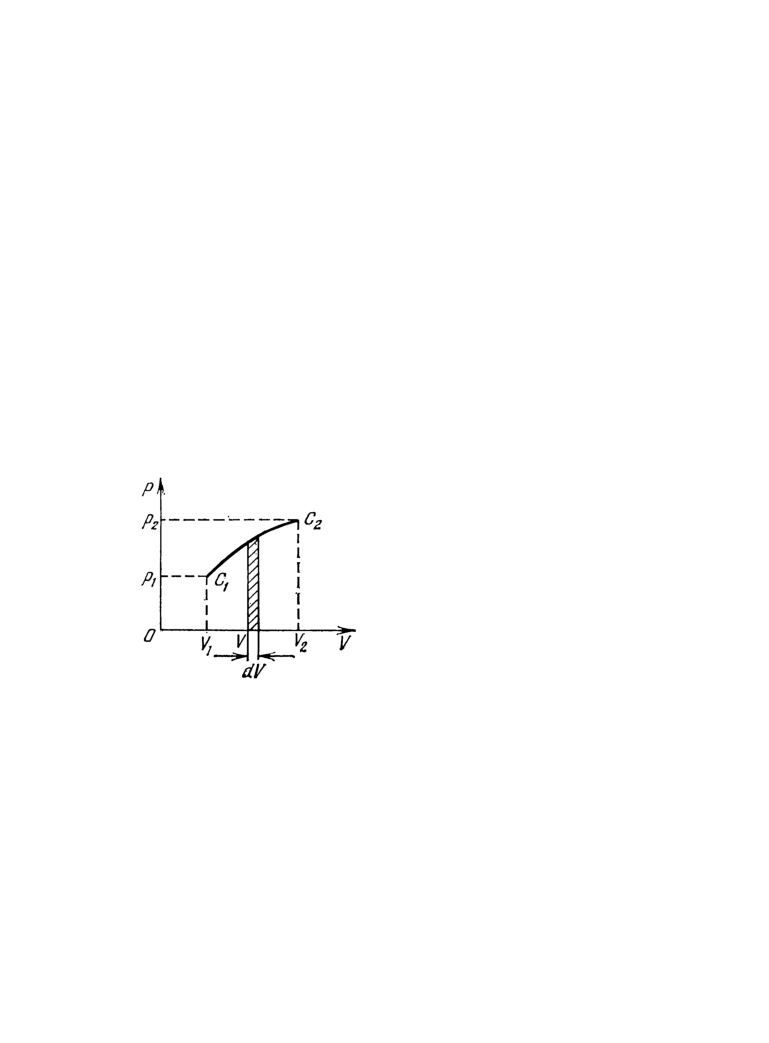
\includegraphics[width=0.8\textwidth]{figs/ch-09/fig-09-02.pdf}
%\input{figs/ch-03/fig-03-01}
%  \vspace{-13pt}
\sidecaption{Graphical representation of an equilibrium process.\zhcap{平衡过程的图示。}\label{fig-09-02}}
\end{marginfigure}

\section[Graphical Representation]{Graphical Representation of Thermodynamic Processes and Work}
\label{sec-9.4}
\zhtitle{热力学过程与功的图示表示}

\subsection{}\label{9.4.1} The equation of state \ssect{8.3.6} of a thermodynamic system enables the value of any state variable, for example $p$, to be determined from any values of two other variables, such as $V$ and $T$. Therefore, thermodynamic processes can be graphically represented in various two-dimensional coordinate systems. In addition to the most extensively used $p V$ diagrams, $p T$ and $V T$ diagrams are also used.
\zhpar{热力学系统的物态方程 \ssect{8.3.6} 使得任一状态参量（例如 $p$）的值可由另外两个参量（例如 $V$ 和 $T$）的值确定。因此，热力学过程可以在各种二维坐标系中用图形表示。除最常用的 $pV$ 图外，$pT$ 图和 $VT$ 图也被广泛使用。}

In \figr{fig-09-02}, the thermodynamic process in the $pV$ diagram is represented by the curve $C_{1}C_{2}$, and the points $C_{1}(p_{1},\, V_{1})$ and $C_{2}(p_{2},\, V_{2})$indicate the initial and final states of the thermodynamic system.
\zhpar{在 \figr{fig-09-02} 中，$pV$ 图中的热力学过程由曲线 $C_{1}C_{2}$ 表示，点 $C_{1}(p_{1},\, V_{1})$ 和 $C_{2}(p_{2},\, V_{2})$ 分别表示热力学系统的初始状态和终末状态。}

Only equilibrium processes \ssect{8.3.7} can be represented graphi­cally. State variables for the whole body (or system) cannot be specified for non-equilibrium processes \ssect{8.3.7} because they differ at different parts of the body (or system). Hence such graphical representation of non-equilibrium processes is impossible.
\zhpar{只有平衡过程 \ssect{8.3.7} 才能用图形表示。对于非平衡过程，由于物体（或系统）的不同部分状态各不相同，无法确定整个物体（或系统）的状态参量，因此非平衡过程不能用这种方式图示。}

\begin{marginfigure}%[!ht]
%\begin{wrapfigure}{r}{0.5\linewidth}
\centering
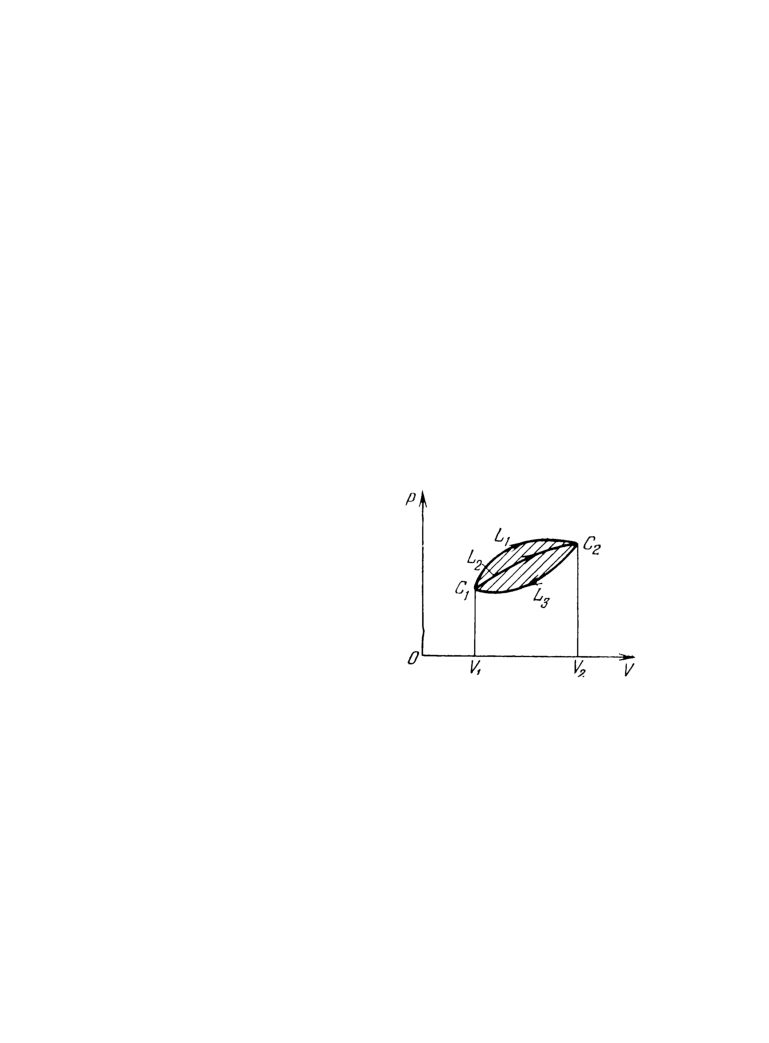
\includegraphics[width=0.8\textwidth]{figs/ch-09/fig-09-03.pdf}
%\input{figs/ch-03/fig-03-01}
%  \vspace{-13pt}
\sidecaption{Finding work done via graphical representation.\zhcap{通过图示法求功。}\label{fig-09-03}}
\end{marginfigure}

\subsection{}\label{9.4.2} An element of work $\delta W$ done by a system \ssect{9.2.3} in an equilibrium process \ssect{8.3.7} can be measured by the area of the trapezoid having one curvilinear side, hatched in \figr{fig-09-02}. The work $W_{1-2}$ done by the system in the process $C_{1}C_{2}$ is equal to
\zhpar{系统在平衡过程 \ssect{8.3.7} 中所做的功元 $\delta W$ \ssect{9.2.3}，可以用\figr{fig-09-02} 中阴影所示的、以一条曲线为一边的梯形面积来度量。系统在过程 $C_{1}C_{2}$ 中所做的功 $W_{1-2}$ 等于}
\begin{equation*}%
W_{1-2} = \int_{V_{1}}^{V_{2}} p \dd V,
\end{equation*}
and is measured by the area that is bounded by the curve re­presenting process $C_{1}C_{2}$,the axis of abscissas and the ordinates $p_{1}$ and $p_{2}$ of points $C_{1}$ and $C_{2}$. The amount of work $W_{1-2}$ done depends on how the system passes from state $C_{1}$ to state $C_{2}$, i.e. upon the kind of process $C_{1}C_{2}$ the system undergoes in changing its state. In the $pV$ diagram of \figr{fig-09-03} the amounts of work done by the system in the processes $C_{1}L_{1}C_{2}$, $C_{1}L_{2}C_{2}$ and $C_{1}L_{3}C_{2}$, and equal to $WL_{1}$, $WL_{2}$ and $WL_{3}$, respectively, are measured by three areas that differ in size: $WL_{1} > WL_{2} > WL_{3}$.
\zhpar{并可由表示过程 $C_{1}C_{2}$ 的曲线、横坐标轴以及点 $C_{1}$ 和 $C_{2}$ 的纵坐标 $p_{1}$ 和 $p_{2}$ 所围成的面积来度量。所做的功 $W_{1-2}$ 取决于系统由状态 $C_{1}$ 变化到状态 $C_{2}$ 的途径，即取决于系统在改变状态时所经历的过程 $C_{1}C_{2}$ 的种类。在 \figr{fig-09-03} 的 $pV$ 图中，系统在过程 $C_{1}L_{1}C_{2}$、$C_{1}L_{2}C_{2}$ 和 $C_{1}L_{3}C_{2}$ 中所做的功分别为 $WL_{1}$、$WL_{2}$ 和 $WL_{3}$，它们分别由三块大小不同的面积来度量，且 $WL_{1} > WL_{2} > WL_{3}$。}

After the system has completed the cycle \ssect{11.1.1} $C_{1}L_{1}C_{2}L_{3}C_{1}$ the total amount of work $W_{C_{1}-C_{1}}$ is not equal to zero. The positive expansion work in process $C_{1}L_{1}C_{2}$ exceeds the negative work done in the compression process $C_{2}L_{3}C_{1}$. The resultant positive work is measured by the hatched area in \figr{fig-09-03}. 
\zhpar{系统完成循环 \ssect{11.1.1} $C_{1}L_{1}C_{2}L_{3}C_{1}$ 后，总功 $W_{C_{1}-C_{1}}$ 不等于零。过程 $C_{1}L_{1}C_{2}$ 中的正膨胀功超过了压缩过程 $C_{2}L_{3}C_{1}$ 中的负功。合成的正功由 \figr{fig-09-03} 中的阴影面积表示。}

\subsection{}\label{9.4.3} The work $W$ and the quantity of heat $Q$ are not state functions \ssect{8.3.8}. In various processes $\hlblue{1} \to \hlblue{2}$, in which the state of a system is changed, various quantities of heat are transferred to the system, and various amounts of work are done. Elements of the changes in the physical quantities $\delta Q$ and $\delta W$ are not complete differentials \ssect{9.1.3}.
\zhpar{功 $W$ 和热量 $Q$ 都不是状态函数 \ssect{8.3.8}。在使系统状态发生变化的各种过程 $\hlblue{1} \to \hlblue{2}$ 中，传递给系统的热量和所做的功各不相同。物理量的变化元 $\delta Q$ 和 $\delta W$ 都不是全微分（参见 \ssect{9.1.3}）。}

\section[Heat Capacity of Matter]{Heat Capacity of Matter. Applying the First Law of Thermodynamics to Isoprocesses in an Ideal Gas}
\label{sec-9.5}
\zhtitle{物质的热容。热力学第一定律在理想气体等过程中的应用}

\subsection{}\label{9.5.1} The \redem{heat capacity} $C$ of a body is a physical quantity, numerically equal to the ratio of the quantity of heat $\delta Q$ transferred to the body to the change $\dd T$ in the temperature of the body in the thermodynamic process being considered:
\zhpar{物体的\redem{热容} $C$ 是一个物理量，其数值等于在所考虑的热力学过程中，传递给物体的热量元 $\delta Q$ 与物体温度的变化元 $\dd T$ 之比：}
\begin{equation*}%
C = \frac{\delta Q}{\dd T}.
\end{equation*}
The value of $C$ depends upon the mass of the body, its chemical composition, thermodynamic state and the process in which the heat $\delta Q$ is transferred to it.
\zhpar{$C$ 的值取决于物体的质量、化学成分、热力学状态，以及传递热量 $\delta Q$ 所经历的过程。}

\subsection{}\label{9.5.2} The \redem{specific heat} $c$ is the heat capacity per unit mass of a substance. For a homogeneous body $c = C/M$, where $M$ is the mass of the body.
\zhpar{\redem{比热容} $c$ 是单位质量物质的热容。对于均匀物体，$c = C/M$，其中 $M$ 为物体的质量。}

The \redem{molar heat capacity} $C_{\mu}$ is the heat capacity of a single mole (Appendix~I) of the substance: $C_{\mu} = \mu \,c$, where $\mu$ is the molar mass \ssect{8.4.3} of the substance.
\zhpar{\redem{摩尔热容} $C_{\mu}$ 是一摩尔（附录~I）物质的热容：$C_{\mu} = \mu \,c$，其中 $\mu$ 为该物质的摩尔质量 \ssect{8.4.3}。}

 
\subsection{}\label{9.5.3} The element of the quantity of heat $\delta Q$ that must be transferred to a body to change its temperature from $T$ to $T + \Delta T$ is
\zhpar{要使物体的温度从 $T$ 变化到 $T + \Delta T$，需要传递给物体的热量元为：}
\begin{equation*}%
\delta Q = C \dd T.
\end{equation*}
For a homogeneous body $\delta Q - M c \,\dd T = (M/\mu) C_{\mu} \dd T$, where $M$ is the mass of the body, $\mu$ is its molar mass and $M/\mu$ is the number of moles in the body. 
\zhpar{对于均匀物体，$\delta Q - M c \,\dd T = (M/\mu) C_{\mu} \dd T$，其中 $M$ 为物体的质量，$\mu$ 为其摩尔质量，$M/\mu$ 为物体中所含的摩尔数。}

\begin{marginfigure}%[!ht]
%\begin{wrapfigure}{r}{0.5\linewidth}
\centering
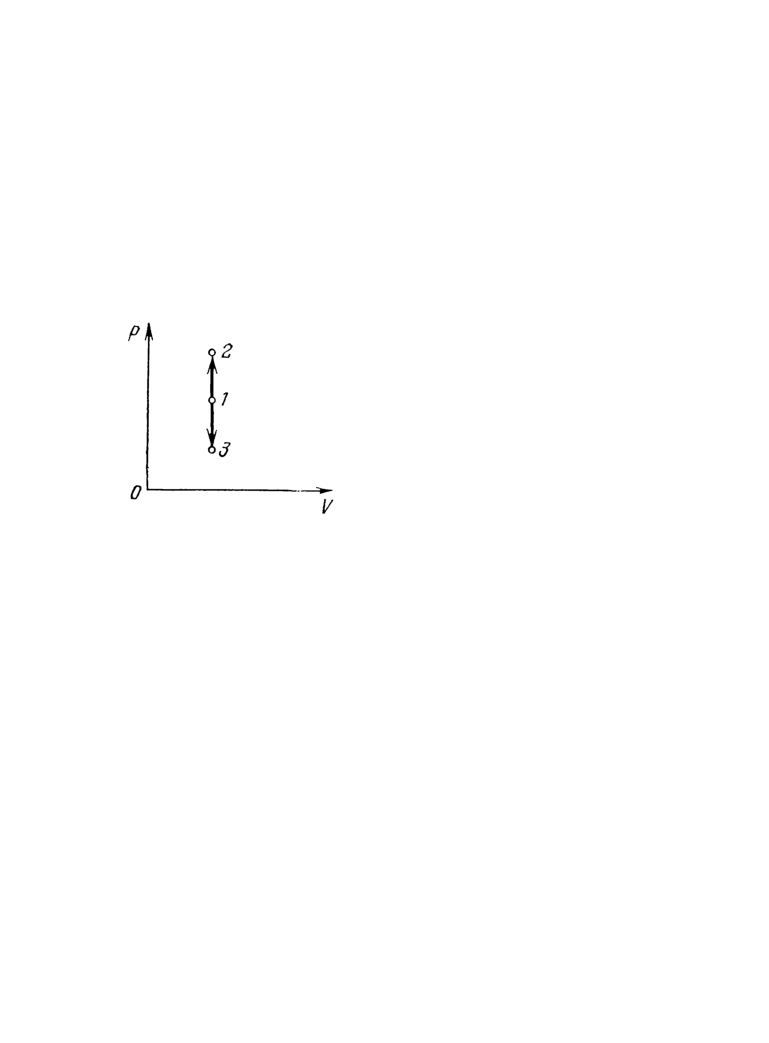
\includegraphics[width=0.8\textwidth]{figs/ch-09/fig-09-04.pdf}
%\input{figs/ch-03/fig-03-01}
%  \vspace{-13pt}
\sidecaption{Finding work done via graphical representation.\zhcap{通过图示法求功。}
\label{fig-09-04}}
\end{marginfigure}

\subsection{}\label{9.5.4} For equilibrium \ssect{8.3.7} iso­ processes in gases \ssect{8.3.7}, the first law of thermodynamics \ssect{9.3.1} is of the form
\zhpar{对于气体的平衡等过程 \ssect{8.3.7}，热力学第一定律 \ssect{9.3.1} 的形式为：}
\begin{equation*}%
\frac{M}{\mu} C_{\mu} \dd T = \dd U + p \dd V.
\end{equation*}
In the isochoric process \ssect{8.3.7}  of heating or cooling a gas (straight lines 1-2 and 1-3 in \figr{fig-09-04}), no element of work $\delta W = p \dd V$ is done (because $\dd V = 0$). The whole quantity of heat trans­ferred to the gas is expended in changing its internal ener­gy: $\delta Q = \dd U$. If $C_{V_{\mu}}$ is the molar heat capacity at constant volume,
\zhpar{在气体的等体加热或冷却过程 \ssect{8.3.7}（\figr{fig-09-04} 中的直线 1-2 和 1-3）中，不做功（因为 $\dd V = 0$，故 $\delta W = p \dd V$ 等于零）。传递给气体的全部热量都用于改变其内能：$\delta Q = \dd U$。若 $C_{V_{\mu}}$ 为定容摩尔热容，则有：}
\begin{equation}%
\frac{M}{\mu} C_{V_{\mu}} \dd T = \dd U + p \dd V.
\tag{$\star$}
\end{equation}
Within a definite temperature range it can be assumed that $C_{V_{\mu}}\approx  \textrm{const}$ (for greater detail see \ssect{10.7.4}) and that the
change in the internal energy of the gas $\Delta U_{1-2}$, as its temper­ature is changed from $T_{1}$ to $T_{2}$, is equal to $\Delta U_{1-2} = U_{2} - U_{1} = (M/\mu) C_{V_{\mu}} (T_{2} - T_{1})$ and is due to the quantity of heat
$Q_{1-2}$ transferred to the gas in the isochoric process:
\zhpar{在一定温度范围内，可以假定 $C_{V_{\mu}}\approx  \textrm{const}$（更详细的内容参见 \ssect{10.7.4}），并且当气体温度从 $T_{1}$ 变化到 $T_{2}$ 时，气体内能的变化 $\Delta U_{1-2} = U_{2} - U_{1} = (M/\mu) C_{V_{\mu}} (T_{2} - T_{1})$，该内能变化是由等体过程中传递给气体的热量 $Q_{1-2}$ 引起的，即：}
\begin{equation}%
Q_{1-2}  = \frac{M}{\mu} C_{V_{\mu}}(T_{2} - T_{1}).
\tag{$\star\star$}
\end{equation}
At $T_{2} > T_{1}$, $Q_{1-2}> 0$ and a definite quantity of heat is trans­ferred to gas; at $T_{2} < T_{1}$, $Q_{1-2} < 0$ and a definite quantity of heat is conducted away from the gas.
\zhpar{当 $T_{2} > T_{1}$ 时，$Q_{1-2}> 0$，有一定量的热量传递给气体；当 $T_{2} < T_{1}$ 时，$Q_{1-2} < 0$，有一定量的热量从气体中导出。}

\subsection{}\label{9.5.5} For an ideal gas, equations $(\star)$ and $(\star\star)$ express the change in its internal energy in \redem{any process} for changing the state of the gas in the temperature range $(T_{2} - T_{1})$. The internal energy of an ideal gas depends only on its chemical composition, mass and temperature.
\zhpar{对于理想气体，式 $(\star)$ 和式 $(\star\star)$ 表示气体在温度区间 $(T_{2} - T_{1})$ 内、在\redem{任意过程}中内能的变化。理想气体的内能仅取决于其化学成分、质量和温度。}

In real gases \ssect{12.1.2} the inter­nal energy includes the poten­tial energy of interaction be­tween the molecules \ssect{9.1.2}, which depends upon the dis­tance between them. This part of the internal energy of a real gas is changed with changes in its volume. Therefore, equations $(\star)$ and $(\star\star)$ express the change in the internal energy of a real gas only when it is heated or cooled in an isochoric (constant-volume) process.
\zhpar{对于实际气体 \ssect{12.1.2}，其内能中包括分子间相互作用的势能 \ssect{9.1.2}，该势能取决于分子之间的距离，因此随气体体积的变化而改变。所以，只有在等体（定容）过程中对实际气体加热或冷却时，式 $(\star)$ 和式 $(\star\star)$ 才能表示其内能的变化。}

\subsection{}\label{9.5.6} In an arbitrary equilibrium process \ssect{8.3.7} that takes place in an ideal gas, the first law of thermodynamics assumes the form
\zhpar{对于理想气体中的任意平衡过程 \ssect{8.3.7}，热力学第一定律的形式为：}
\begin{equation*}%
\frac{M}{\mu} C_{\mu}\dd T = \frac{M}{\mu} C_{V_{\mu}} \dd T + p \dd V,
\end{equation*}
where $C_{\mu}$ is the molar heat capacity of an ideal gas in the given process. The isobaric process \ssect{8.3.7} of heating (straight line 1-2 in \figr{fig-09-05}) or cooling (straight line 1-3 in \figr{fig-09-05}) a gas can be carried out, for instance, in a vessel (cylinder) closed by a movable piston subject to a constant external pressure. An clement of work 6IF done by an ideal gas in an isobaric process is
\zhpar{式中 $C_{\mu}$ 为理想气体在该过程中的摩尔热容。气体的等压加热（\figr{fig-09-05} 中的直线 1-2）或冷却（\figr{fig-09-05} 中的直线 1-3）过程，例如可以在一个由可动活塞封闭、外部压强恒定的容器（气缸）中进行。理想气体在等压过程中所做的功元为：}
\begin{equation*}%
\delta W = p \dd V = \frac{M}{\mu} R \dd T,
\end{equation*}
in which use is made of the expression $\dd V = (M/\mu) (R/p) \dd T$ from the Mendeleev-Clapeyron equation \ssect{8.4.4} at $p = \textrm{const}$.
\zhpar{式中利用了在 $p = \textrm{const}$ 时由门捷列夫-克拉珀龙方程 \ssect{8.4.4} 得到的关系式 $\dd V = (M/\mu) (R/p) \dd T$。}
\begin{marginfigure}[-4cm]%[!ht]
%\begin{wrapfigure}{r}{0.5\linewidth}
\centering
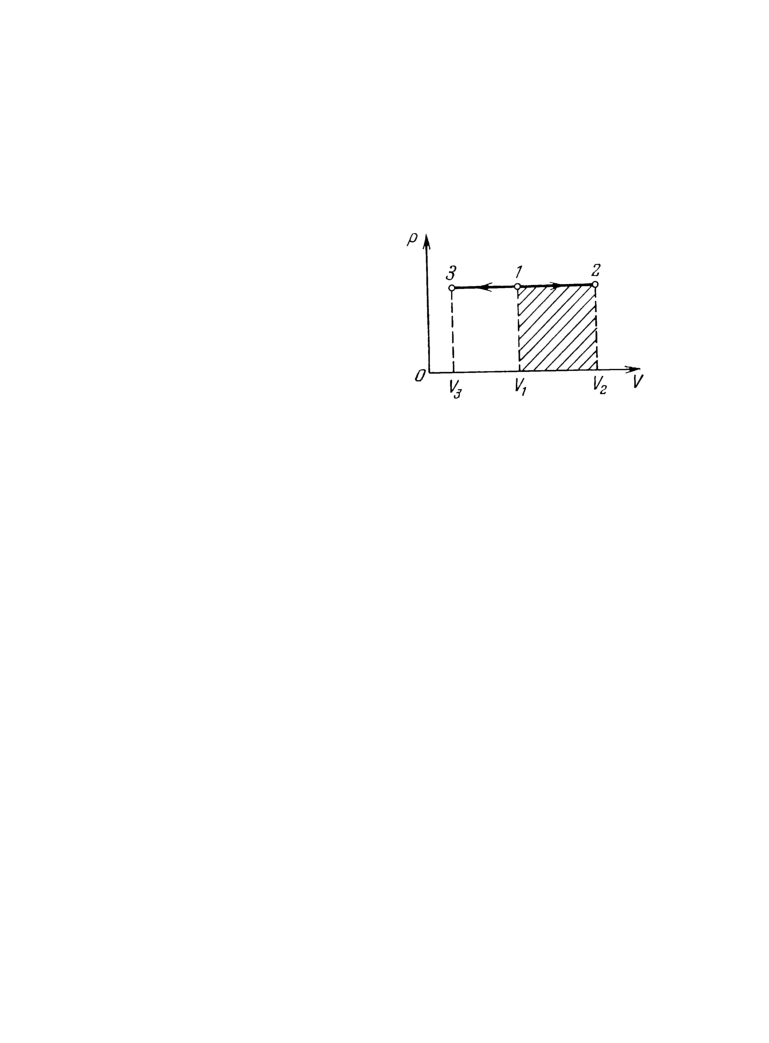
\includegraphics[width=0.8\textwidth]{figs/ch-09/fig-09-05.pdf}
%\input{figs/ch-03/fig-03-01}
%  \vspace{-13pt}
\sidecaption{Finding work done via graphical representation.\zhcap{通过图示法求功。}\label{fig-09-05}}
\end{marginfigure}
The universal gas constant $R$ \ssect{8.4.4} is numerically equal to the work done by one mole of an ideal gas when it is heated isobarically by one degree:
\zhpar{摩尔气体常量 $R$ \ssect{8.4.4} 在数值上等于一摩尔理想气体在等压下升高一度时所做的功：}
\begin{equation*}%
R = \frac{\delta W}{(M/\mu) \dd T }.
\end{equation*}
The work $W_{1-2}$ done by the gas in isobaric expansion 1-2 is
\zhpar{气体在等压膨胀过程 1-2 中所做的功 $W_{1-2}$ 为：}
\begin{equation*}%
W_{1-2} = \int_{V_{1}}^{V_{2}} p \dd V = p (V_{2} - V_{1}).
\end{equation*}
It is represented by the hatched area in \figr{fig-09-05}. For an ideal gas the work $W_{1-2}$ is also equal to
\zhpar{该功由 \figr{fig-09-05} 中的阴影面积表示。对于理想气体，功 $W_{1-2}$ 也等于：}
\begin{equation*}%
W_{1-2} = \frac{M}{\mu} R (T_{2} - T_{1}).
\end{equation*}


\subsection{}\label{9.5.7} The element of the quantity of heat $\delta Q$ transferred to the gas in the isobaric process is
\zhpar{气体在等压过程中所吸收的热量元 $\delta Q$ 为：}
\begin{equation*}%
\delta Q = \frac{M}{\mu} C_{p\mu} \dd T,
\end{equation*}
where $C_{p\mu}$ is the molar heat capacity at constant pressure. If the quantity $C_{p\mu}$ can be assumed constant in the temperature
range $(T_{2} - T_{1})$ then the quantity of heat $Q_{1-2}$ transferred to (or conducted away from) the gas is
\zhpar{式中 $C_{p\mu}$ 为定压摩尔热容。若在温度区间 $(T_{2} - T_{1})$ 内可以认为 $C_{p\mu}$ 为常量，则传递给气体（或从气体中导出）的热量 $Q_{1-2}$ 为：}
\begin{equation*}%
Q_{1-2} = \frac{M}{\mu} C_{p\mu} (T_{2} - T_{1}).
\end{equation*}

\subsection{}\label{9.5.8} The molar heat capacities $C_{p\mu}$ and $C_{V\mu}$ of a gas are re­lated by the \redem{Mayer equation}
\zhpar{气体的定压摩尔热容 $C_{p\mu}$ 与定容摩尔热容 $C_{V\mu}$ 满足\redem{迈耶方程}：}
\begin{equation*}%
C_{p\mu} - C_{V\mu} = R.
\end{equation*}
For specific heats $c_{p}$ and $c_{V}$, the Mayer relation is of the form 
\zhpar{对于比热容 $c_{p}$ 和 $c_{V}$，迈耶关系式的形式为：}
\begin{equation*}%
c_{p} - c_{V} = \frac{R}{\mu},
\end{equation*}
where $\mu$ is the molar mass \ssect{8.4.3} of the gas. 
\zhpar{式中 $\mu$ 为气体的摩尔质量 \ssect{8.4.3}。}

For the heat capacities $C_{p}$ and $C_{V}$
\zhpar{对于热容 $C_{p}$ 和 $C_{V}$，有：}
\begin{equation*}%
C_{p} - C_{V} = \frac{M}{\mu} R,
\end{equation*}
where $M$ is the mass of the gas and $M/\mu$ is the number of moles it contains.
\zhpar{式中 $M$ 为气体的质量，$M/\mu$ 为其所含的摩尔数。}

The Mayer relation indicates that in heating a gas isobarically by one degree a greater quantity of heat must be transferred to the gas than in isochoric heating by the same amount. This difference between the quantities of heat should be equal to the work done by the gas in its isobaric expansion. 
\zhpar{迈耶关系表明，使气体等压升高一度所需传递的热量，比使其等体升高相同温度所需传递的热量要多。这两部分热量之差，应等于气体在等压膨胀过程中所做的功。}


\subsection{}\label{9.5.9} The isothermal process \ssect{8.3.7} of expanding (or compressing) a gas takes place in heat exchange \ssect{9.2.4} between the gas and the external me­dium at a constant tempera­ture difference. For this to be feasible, the heat capacity \ssect{9.5.1} of the external medium should be sufficiently great and the process of expansion (or compression) should proceed extremely slowly. First-order phase transitions \ssect{12.3.3}, such as boiling and condensa­tion, are isothermal processes if they proceed at constant ex­ternal pressure.
\zhpar{气体的等温膨胀（或压缩）过程 \ssect{8.3.7} 是在气体与外部介质之间进行热交换 \ssect{9.2.4} 的过程中实现的，且两者的温差保持恒定。要使这一过程得以实现，外部介质的热容 \ssect{9.5.1} 应足够大，并且膨胀（或压缩）过程必须极其缓慢地进行。一级相变 \ssect{12.3.3}（例如沸腾和凝结）在外部压强恒定时进行，也是等温过程。}

In an isothermal process in an ideal gas the internal energy of the gas remains unchanged \ssect{9.5.5} and the whole quantity of heat $Q_{1-2}$ transferred to the gas is expended in the work $W_{1-2}$ done by the gas to overcome the external forces:
\zhpar{在理想气体的等温过程中，气体的内能保持不变 \ssect{9.5.5}，传递给气体的全部热量 $Q_{1-2}$ 都用于气体克服外力所做的功 $W_{1-2}$：}
\begin{equation*}%
Q_{1-2} = W_{1-2} = \int_{V_{1}}^{V_{2}} p \dd V = \frac{M}{\mu} RT \int_{V_{1}}^{V_{2}} \frac{\dd V}{V} =\frac{M}{\mu} RT \ln \frac{V_{2}}{V_{1}}.
\end{equation*}
Here $\frac{M}{\mu}$ is the number of moles contained in mass $M$ of the gas, $T$ is the constant temperature of the gas, and $V_{1}$ and $V_{2}$ are the initial and final volumes of the gas. If the gas isother­mally expands $(V_{2}> V_{1})$, heat is being transferred to it $Q_{1-2}> 0$)and it is doing positive work $(W_{1-2} > 0)$ represented by the hatched area in \figr{fig-09-06}. 
\zhpar{此处 $\frac{M}{\mu}$ 为质量为 $M$ 的气体所含的摩尔数，$T$ 为气体恒定的温度，$V_{1}$ 和 $V_{2}$ 分别为气体的初始体积和终末体积。若气体等温膨胀（$V_{2}> V_{1}$），则有热量传递给气体（$Q_{1-2}> 0$），且气体做正功（$W_{1-2} > 0$），其大小由 \figr{fig-09-06} 中的阴影面积表示。}
\begin{marginfigure}%[!ht]
%\begin{wrapfigure}{r}{0.5\linewidth}
\centering
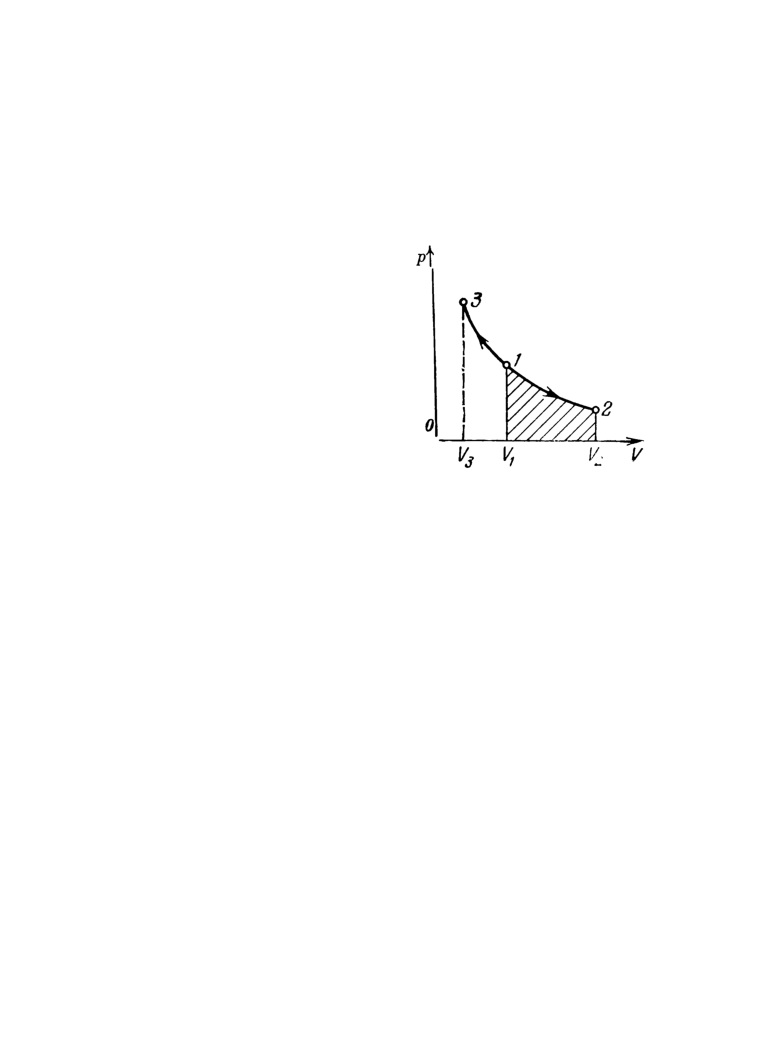
\includegraphics[width=0.8\textwidth]{figs/ch-09/fig-09-06.pdf}
%\input{figs/ch-03/fig-03-01}
%  \vspace{-13pt}
\sidecaption{Finding work done via graphical representation.\zhcap{通过图示法求功。}
\label{fig-09-06}}
\end{marginfigure}
In isothermal compression of the gas (process 1-3 in \figr{fig-09-06}), the work done by the gas is negative $(W_{1-3} < 0)$ . Positive work $(W_{1-3}' = -W_{1-3}> 0)$ is being done by the external forces to compress the gas. In com­pression, a certain quantity of heat is conducted away from the gas $(Q_{1-3} < 0)$. The heat capacity of a substance in an isother­mal process equals infinity ($\dd T = 0$ and $\delta Q \neq 0$).
\zhpar{在气体的等温压缩过程（\figr{fig-09-06} 中的过程 1-3）中，气体所做的功为负（$W_{1-3} < 0$）。外力压缩气体时做正功（$W_{1-3}' = -W_{1-3}> 0$）。压缩过程中，一定量的热量从气体中导出（$Q_{1-3} < 0$）。物质在等温过程中的热容等于无穷大（$\dd T = 0$ 且 $\delta Q \neq 0$）。}

\subsection{}\label{9.5.10} An adiabatic process \ssect{8.3.7} proceeds under the condition that $\delta Q  = 0$. It is essential that the condition $Q = 0$ does not define this process, because it does not specify the absence of heat exchange with the external medium. It only indicates that the algebraic sum of the quantities of heat transferred to and conducted away from the gas in various parts of the process equals zero. In an adiabatic process, work is done by an ideal gas at the expense of its internal energy:
\zhpar{绝热过程 \ssect{8.3.7} 在 $\delta Q  = 0$ 的条件下进行。需要指出，条件 $Q = 0$ 并不能定义绝热过程，因为它并不说明系统与外部介质之间没有热交换，而只说明在过程的各个阶段传递给气体和从气体中导出的热量的代数和为零。在绝热过程中，理想气体靠消耗其内能做功：}
\begin{equation*}%
\delta W = - \dd U = -\frac{M}{\mu} C_{V\mu} \dd T,
\end{equation*}
where $C_{V\mu}$ is the molar heat capacity of the gas at constant volume, $M/\mu$ is the number of moles contained in mass $M$ of the gas, and $\dd T$ is an element of change in the temperature of the gas. If the gas adiabatically expands $(\delta W = p \dd V > 0)$, it is cooled $(\dd T < 0)$. In adiabatic compression the gas is heated: $\delta W = p \dd V < 0$ and $\dd T > 0$.
\zhpar{式中 $C_{V\mu}$ 为气体的定容摩尔热容，$M/\mu$ 为质量为 $M$ 的气体所含的摩尔数，$\dd T$ 为气体温度的变化元。若气体绝热膨胀（$\delta W = p \dd V > 0$），则其温度降低（$\dd T < 0$）。绝热压缩时，气体被加热：$\delta W = p \dd V < 0$，且 $\dd T > 0$。}

\subsection{}\label{9.5.11} The \redem{adiabatic}, or \redem{Poisson, equation}: $pV^{\varkappa}= \textrm{const}$, is valid for an equilibrium adiabatic process \ssect{8.3.7}.
\zhpar{\redem{绝热方程}，即\redem{泊松方程}：$pV^{\varkappa}= \textrm{const}$，适用于平衡绝热过程 \ssect{8.3.7}。}

\begin{marginfigure}%[!ht]
%\begin{wrapfigure}{r}{0.5\linewidth}
\centering
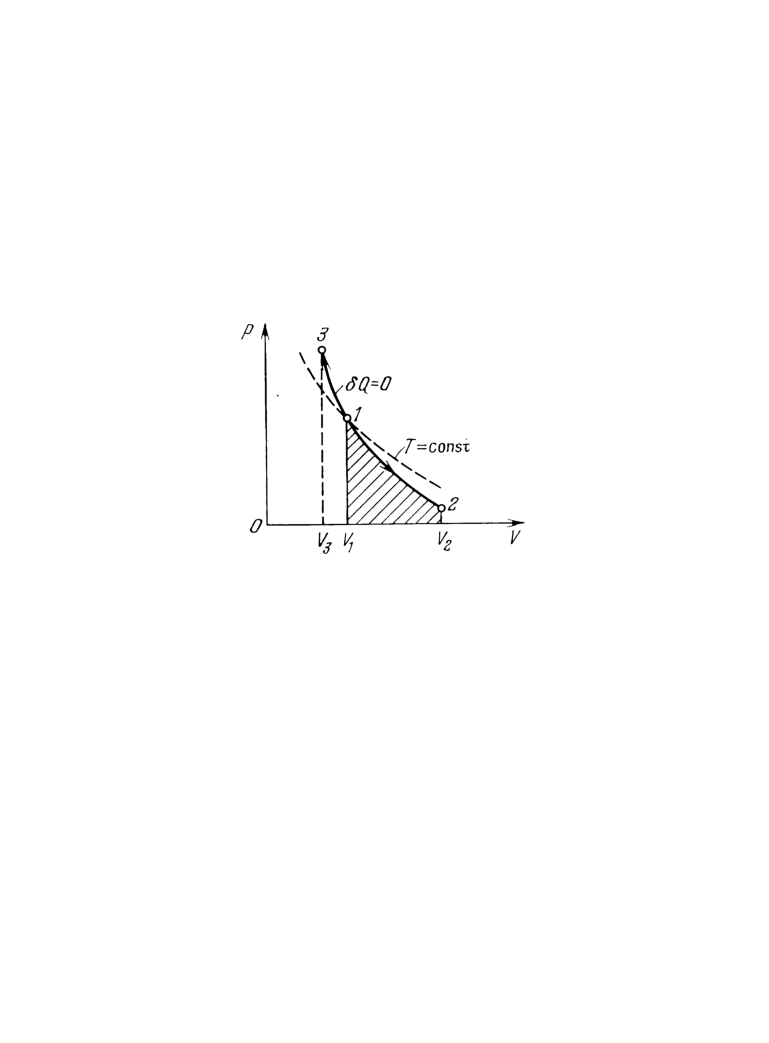
\includegraphics[width=0.8\textwidth]{figs/ch-09/fig-09-07.pdf}
%\input{figs/ch-03/fig-03-01}
%  \vspace{-13pt}
\sidecaption{Finding work done via graphical representation.\zhcap{通过图示法求功。}\label{fig-09-07}}
\end{marginfigure}


Making use of the Mendeleev-Clapeyron equation \ssect{8.4.4}, the relation between $p$ and $T$, and also between $V$ and $T$, in an adiabatic process can be found from the adiabatic equation:
\zhpar{利用门捷列夫-克拉珀龙方程 \ssect{8.4.4}，可由绝热方程求出绝热过程中 $p$ 与 $T$ 之间以及 $V$ 与 $T$ 之间的关系：}
\begin{equation*}%
pT^{\frac{\varkappa}{\varkappa -1}} = \textrm{const.}, \qand VT^{\frac{1}{\varkappa -1}}= \textrm{const}.
\end{equation*}
In these equations the dimensionless quantity $\varkappa = C_{p\mu}/C_{V\mu}$ $= c_{p}/c_{V} > 1$ is the \redem{adiabatic exponent}. The full curve in \figr{fig-09-07}, called an \redem{adiabat} or \redem{adiabatic curve}, represents an adiabatic process in a $pV$ diagram. The dashed curve on this diagram, called an \redem{isotherm}, represents an isothermic process at the temperature corresponding to the initial state \hlblue{1} of the gas. In an adiabatic process the pressure varies with the volume more rapidly than in an isothermic process (the curve is steep­ er). 
\zhpar{式中，无量纲量 $\varkappa = C_{p\mu}/C_{V\mu}$ $= c_{p}/c_{V} > 1$ 称为\redem{绝热指数}。\figr{fig-09-07} 中的实线称为\redem{绝热线}或\redem{绝热曲线}，表示 $pV$ 图中的绝热过程。图中的虚线称为\redem{等温线}，表示温度与气体初始状态 \hlblue{1} 的温度相同的等温过程。在绝热过程中，压强随体积的变化比在等温过程中更为迅速（曲线更陡）。}

In adiabatic expansion the temperature of the gas and its pressure decrease faster than in the corresponding isothermal expansion. In adiabatic compression of the gas its pressure increases at a higher rate than in the corresponding isothermal compression. The reason is that the increased pressure is due both to the decrease in the volume of the gas and to the increase in its temperature.
\zhpar{绝热膨胀时，气体的温度和压强的降低比相应的等温膨胀更快。绝热压缩时，气体压强的增加比相应的等温压缩更快。原因在于，压强的增大既是由于气体体积减小，也是由于其温度升高。}

\subsection{}\label{9.5.12} The work $W_{1-2}$ done by the gas in the adiabatic process $\hlblue{1} \to \hlblue{2}$ is measured by the hatched area in \figr{fig-09-07}.
\zhpar{绝热过程 $\hlblue{1} \to \hlblue{2}$ 中气体所做的功 $W_{1-2}$，由 \figr{fig-09-07} 中的阴影面积表示。}

The amount of work $W_{1-2}$ done in an adiabatic process is ex­pressed by
\zhpar{绝热过程中所做的功 $W_{1-2}$ 可表示为：}


In these equations $M/\mu$ is the number of moles contained in mass $M$ of the gas, $C_{V\mu}$ is the molar heat capacity at constant volume, $\varkappa$ is the adiabatic exponent, and $p$, $V$ and $T$ are the state variables of the gas in the states \hlblue{1} and \hlblue{2} as indicated.
\zhpar{式中 $M/\mu$ 为质量为 $M$ 的气体所含的摩尔数，$C_{V\mu}$ 为定容摩尔热容，$\varkappa$ 为绝热指数，$p$、$V$ 和 $T$ 为气体在所示状态 \hlblue{1} 和 \hlblue{2} 中的状态参量。}

\subsection{}\label{9.5.13} \tabl{table-9.1} lists summarized information on the isoprocesses in gases.
\zhpar{\tabl{table-9.1} 汇总列出了气体等过程的相关信息。}

\clearpage
%\begin{landscape}

\begin{table*}
\begin{scriptsize}
\begin{tabular}{p{1.5cm}p{2cm}p{2cm}p{2.2cm}p{2.5cm}}
\toprule
\hlblue{Thermodynamic Process} & \hlblue{Isochoric} & \hlblue{Isobaric} & \hlblue{Isothermal} & \hlblue{Adiabatic} \\
\midrule
Basic Condition & $V = \textrm{const.}$  & $p = \textrm{const.}$  & $T = \textrm{const}$  & $\delta Q = 0$ \\ 
\midrule
Relationship between state variables & $\dfrac{p}{T} = \textrm{const.}$ & $\dfrac{V}{T} =  \textrm{const}$ & $pV = \textrm{const.}$ &  $pV^{\varkappa} = \textrm{const.}$ \\
& & & &  $pT^{\varkappa/(\varkappa -1)} = \textrm{const.}$\\
& & & &  $VT^{1/(\varkappa -1)} = \textrm{const.}$\\
\midrule
Work done in the process& $\delta W  = 0 $ & $\delta W = p \dd V$ &$\delta W = p \dd V$& $\delta W = p \dd V \newline  = -\dd U$ \\
&  $ W  = 0 $& $W = p (V_{2} - V_{1})$ & $W = \dfrac{M}{\mu} RT \ln\dfrac{V_{2}}{V_{1}}$ & $W = -\Delta U \newline = C_{V} (T_{2} - T_{1})$\\
\midrule
Quantity of heat transferred in the process& $\delta Q  = C_{V} \dd T $& $\delta Q = C_{p} \dd T$ & $\delta Q = \delta W$& $\delta Q = 0$ \\
& $Q = C_{V} (T_{2} - T_{1})$ & $Q = C_{p} (T_{2} - T_{1})$ & $Q =W$& $Q = 0$\\
\midrule
Change in internal energy& $\dd U  = \delta Q $ & $\dd U  = C_{V} \dd T $& $\dd U =0$ & $\dd U = - \delta W \newline  = C_{V} \dd T$ \\
& $U=Q$ & $U = C_{V}(T_{2} - T_{1})$& $\Delta U = 0$ & $\Delta U = -W \newline = C_{V} (T_{2} - T_{1})$ \\
\midrule
Heat capacity& $C_{V} = \dfrac{M}{\mu}\dfrac{R}{\varkappa -1}$&$C_{p} = \dfrac{M}{\mu}\dfrac{\varkappa R}{\varkappa -1}$ & $C_{T}=\infty$ & $C_{ad}=0$\\
\bottomrule
\end{tabular}
\end{scriptsize}
\caption{A table of isoprocesses.\zhcap{等过程汇总表。}
\label{table-9.1}}
\end{table*}
%\end{landscape}